% !TeX program = pdfLaTeX
\documentclass[12pt]{article}
\usepackage{amsmath}
\usepackage{graphicx,psfrag,epsf}
\usepackage{enumerate}
\usepackage{natbib}
\usepackage{textcomp}
\usepackage[hyphens]{url} % not crucial - just used below for the URL
\usepackage{hyperref}

%\pdfminorversion=4
% NOTE: To produce blinded version, replace "0" with "1" below.
\newcommand{\blind}{0}

% DON'T change margins - should be 1 inch all around.
\addtolength{\oddsidemargin}{-.5in}%
\addtolength{\evensidemargin}{-.5in}%
\addtolength{\textwidth}{1in}%
\addtolength{\textheight}{1.3in}%
\addtolength{\topmargin}{-.8in}%

%% load any required packages here



% tightlist command for lists without linebreak
\providecommand{\tightlist}{%
  \setlength{\itemsep}{0pt}\setlength{\parskip}{0pt}}



\usepackage[dvipsnames]{xcolor} % colors
\newcommand{\aak}[1]{{\textcolor{blue}{#1}}}
\newcommand{\svp}[1]{{\textcolor{RedOrange}{#1}}}
\newcommand{\yg}[1]{{\textcolor{Green}{#1}}}
\usepackage[capitalise]{cleveref}
\newcommand\pcref[1]{(\cref{#1})}
\usepackage{algorithm,algpseudocode,booktabs}
\usepackage{booktabs}
\usepackage{longtable}
\usepackage{array}
\usepackage{multirow}
\usepackage{wrapfig}
\usepackage{float}
\usepackage{colortbl}
\usepackage{pdflscape}
\usepackage{tabu}
\usepackage{threeparttable}
\usepackage{threeparttablex}
\usepackage[normalem]{ulem}
\usepackage{makecell}
\usepackage{xcolor}

\begin{document}


\def\spacingset#1{\renewcommand{\baselinestretch}%
{#1}\small\normalsize} \spacingset{1}


%%%%%%%%%%%%%%%%%%%%%%%%%%%%%%%%%%%%%%%%%%%%%%%%%%%%%%%%%%%%%%%%%%%%%%%%%%%%%%

\if0\blind
{
  \title{\bf A Spatio-Temporal Model for Arctic Sea Ice}

  \author{
        Alison Kleffner \\
    Department of Statistics, University of Nebraska - Lincoln\\
     and \\     Susan VanderPlas \\
    Department of Statistics, University of Nebraska - Lincoln\\
     and \\     Yawen Guan \\
    Department of Statistics, University of Nebraska - Lincoln\\
      }
  \maketitle
} \fi

\if1\blind
{
  \bigskip
  \bigskip
  \bigskip
  \begin{center}
    {\LARGE\bf A Spatio-Temporal Model for Arctic Sea Ice}
  \end{center}
  \medskip
} \fi

\bigskip
\begin{abstract}
Arctic Sea Ice is a barrier between the warm air of the ocean and the
atmosphere, thus playing an important role in the climate. When narrow
linear cracks (leads) form in the sea ice, the heat from the ocean is
released into the atmosphere. To estimate where leads may form, motion
data from the RADARSAT Geophysical Processing System (RGPS) is analyzed.
RGPS provides a set of trajectories of points on the ice sheet to trace
the displacement of sea ice, however, chunks of data are missing due to
collecting data by satellite. We propose a spatio-temporal clustering
and interpolation method that estimates where a lead may form and allows
us to infer missing observations. Features based on the sea ice
displacement are created for k-means clustering by creating a bounding
box around each trajectory, resulting in trajectories being assigned a
cluster. A lead is considered to have formed on the boundary between
different clusters. Using the clusters, a spatio-temporal interpolation
model using a Gaussian Process is used to infer missing locations. Our
clustering approach is compared to ice lead detection methods, and
cross-validation is used to assess our interpolation method.
\end{abstract}

\noindent%
{\it Keywords:} spatial clustering, non-stationary, Gaussian process
\vfill

\newpage
\spacingset{1.45} % DON'T change the spacing!

\hypertarget{intro}{%
\section{Introduction}\label{intro}}

Sea ice in the Arctic Ocean acts as an insulator between the warm ocean
and the cooler atmosphere \citep{peterson_evaluating_2011}. However, sea
ice is constantly changing and moving due to dynamic processes,
including wind and ocean currents, which causes ice cracks, also called
leads, in the ice to form
\citep{peterson_evaluating_2011, hoffman_detection_2019, hutter_leads_2019}.
When a lead forms in the sea ice it provides a significant source of
heat and moisture into the atmosphere, which reduces the overall sea ice
concentration, and warms the regional atmospheric boundary layer
\citep{key_detectability_1993, reiser_new_2020}. Additionally, the
formation of leads has an affect on atmosphere and ocean chemical
exchanges, which include carbon dioxide and mercury
\citep{hoffman_detection_2019}. Thus, the state of the sea ice,
including lead characteristics, provides important information for
weather prediction, climate models, and ocean models
\citep{reiser_new_2020}. When leads form, this may be an indicator of
climate change, and may also be a driver of climate change due to the
release of warmer air \citep{peterson_evaluating_2011}.

Current methods to determine the location of leads generally involve
either the use of thermal infrared satellite data or the calculation of
ice deformation. Thermal methods tend to use thermal channels from the
Advanced Very High Resolution Radiometer (AVHRR), as the surface
temperatures between a lead and the surrounding sea ice are different
\citep{key_detectability_1993}. Using thermal channels from the AVHRR is
highly dependent on clear skies, as clouds can also give a higher
temperature reading and may be mistaken for a lead. Methods have been
suggested to reduce the impact of clouds.
\citet{willmes_pan-arctic_2015} used only clear sky pixels from the
Moderate Resolution Imagery Spectroradtiometer (MODIS). However, MODIS
has issues with low and thin clouds. Hence, a fuzzy cloud artifact
filter was used to remove any remaining clouds, but there is a trade-off
between parameterization and error rates. \citet{rohrs_algorithm_2012}
suggested using passive microwave data as clouds are transparent at
microwave wavelengths. However, microwave data lacks wide spatial
coverage and has coarse resolution making detecting narrow leads
impossible \citep{hoffman_detection_2019}.

Deformation methods to locate leads is determined by the motion of sea
ice. These methods use NASA's RADARSTAT Geophysical Processing System
(RGPS), which uses synthetic aperture radar (SAR) images to track the
trajectory of points on Arctic sea ice. To track trajectories, points
are initially assigned to a vertex of a grid cell on sea ice, which is
tracked over time using the SAR satellite images. Then the deformation
of the ice is calculated within each grid cell, where areas of high
deformation may be denoted as leads \citep{peterson_evaluating_2011}.
These methods can provide additional information about a lead, such as
size and deformation. However, satellites only pass over the same area
every three to six days, so we do not have a complete set of space-time
observations to calculate deformation. Additionally, the error in the
deformation calculations may be strongly underestimated as the grid
cells may become distorted due to movement, which affects deformation
calculations \citep{bouillon_producing_2015}.

Satellite-derived data used to monitor dynamic items, such as the ocean
surface, can have large missing data rates either due to the sampling
rate of atmospheric conditions \citep{fablet_data-driven_2017}. Thus, if
we want to have complete gridded data, interpolation is necessary. When
working with dynamic data the spatio-temporal dynamics need to be
reconstructed in order to interpolate. In optimal interpolation, the
covariance function of the spatio-temporal field-dynamics is used. The
interpolated field is a result of a linear combination of the
observations, assuming stationarity
\citep{fablet_data-driven_2017, ouala_neural_2018}. Additionally, due to
large amounts of data being collected, data driven methods have become
popular. For example, data assimilation involves the construction of a
dynamical systems made using the data
\citep{li_variational_2015, fablet_data-driven_2017, ouala_neural_2018}.

Often when working with data relating to the environment, a simple
global mean and covariance function is inaccurate as the relationships
between variables may change over space. Hence, when developing a
non-stationary spatio-temporal model, the mean and covariance function
should have different parameters depending on the region. Therefore, a
non-stationary model can be developed, either through a Gaussian Process
or Bayesian Hierarchical framework, where the covariance function
parameters varies by different regions
\citep{guinness_nonstationary_2013, SALVANA2020100411}.

Our proposed method for lead detection uses the movement of the sea ice.
However, we want to use the knowledge that sea ice movement is not
consistent, as the underlying process will cause the sea ice to move
differently depending on the location resulting in leads
\citep{peterson_evaluating_2011}. Thus, we aim to determine lead
location by finding clusters of similar movement, where the boundaries
between the clusters are the location of leads. Additionally, using the
information gained from clustering, we developed a non-stationary
spatio-temporal interpolation method to estimate missing points along a
trajectory. Within a cluster, all trajectories move in a similar
fashion, so would expect a missing point to move similarly to observed
points in the cluster. Hence, we can then create a completely gridded
data set that can be used to calculate deformation.

\hypertarget{data}{%
\section{Data}\label{data}}

Data on the movement of the sea ice comes from NASA's RADARSTAT
Geophysical Processing System (RGPS). RGPS data is useful as it is
independent of cloud coverage and has broad spatial coverage.
Trajectories of around 30,000 points are tracked by RGPS using
sequential synthetic aperture radar (SAR) images on the Arctic sea ice
\citep{lindsay_radarsat_2003}. To track these points, an initial grid is
created at the start of the study period where each cell dimension is 10
km on a side \citep{kwok_seasonal_2002}. The vertex of each cell is
assigned an identifier \(g\). In each SAR image, the points are found
again using area-based and feature-based tracking
\citep{peterson_evaluating_2011}. The trajectories of each identifier
\(g\) form a set of all trajectories
\(\mathcal{G} =\left\{g_1,...,g_n\right\}\), where
\(g_j = \left\{\textbf{s}_{jt}: t \in \mathcal{T}_j\right\}\). The
location of \(g_j\) is represented as
\(\textbf{s}_{jt} = (x_{jt}, y_{jt})^T\) or a set of latitude and
longitude. Most \(g_j\) are tracked in three day intervals, however
sampling can be irregular \citep{peterson_evaluating_2011}. Thus,
\(\mathcal{T}_j \subset \left\{1,...,T\right\}\) is a collection of time
points where identifier \(g_j\) is observed. We focus on the Beaufort
region, which has n = 8811 and \(T\)=22.

\begin{figure}[tbp]

{\centering 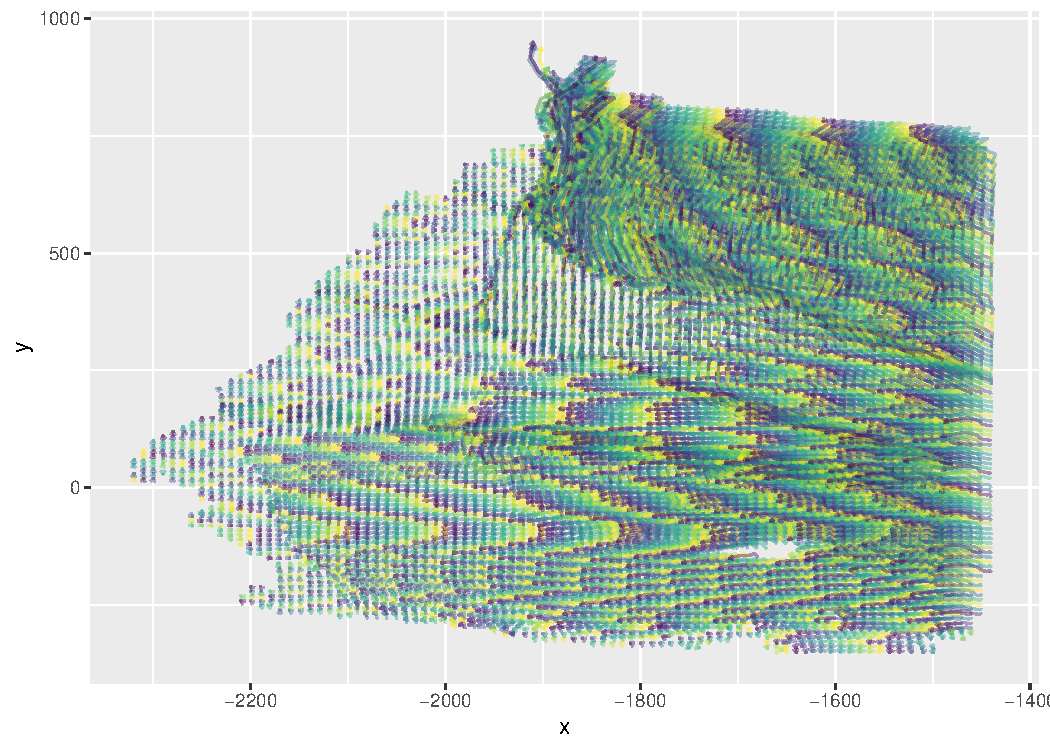
\includegraphics[width=\linewidth,]{spatio-temporal-model-arctic-sea-ice_files/figure-latex/trajectories-1} 

}

\caption{Plot of observed trajectories of sea ice movement. Each trajecotry is rperesented by a line with an arrow to indicate the direction of movement. To help visually distinguish the individual trajectories, multiple colors were used for the trajectories}\label{fig:trajectories}
\end{figure}

Since we want to detect leads only using movement data, it is first
important to visualize the movement. Thus, a plot of the trajectory of
each \(g_j\) is found in \cref{fig:trajectories}. This figure shows that
groups of trajectories appear to move with similar patterns. For
instance, at the top of \cref{fig:trajectories}, a group of trajectories
are traveling upwards, while in the middle a group is traveling from
right to left. Visualizing the movement led to the idea of clustering
similar trajectories, since the similar movement happens in continguous
patches. The movement of each trajectory can be summarized by creating a
bounding box around the trajectory. This allows for the creation of
features that can be used in a clustering algorithm, and it
circumnavigates the missing data issue. After the bounding box features
are created, the trajectories are grouped with other that have similar
features. Leads are considered to be location on the boundary between
groups, as these groups are moving differently.

\hypertarget{methods}{%
\section{Methods}\label{methods}}

\hypertarget{spatio-temporal-clustering-bounding-box}{%
\subsection{Spatio-Temporal Clustering: Bounding
Box}\label{spatio-temporal-clustering-bounding-box}}

\hypertarget{bounding-box-features}{%
\subsubsection{Bounding Box Features}\label{bounding-box-features}}

The bounding box that is created around each trajectory is used to
derive features that represent it's movement. Features includes the
length traveled between the minimum and maximum location of a coordinate
(\(x_{max} - x_{min}\) and \(y_{max} - y_{min}\)), representing the
total distance traveled. However, the maximum and minimum locations may
not always correspond to the first and last day of the time frame.
Hence, the difference in each coordinate (\(x_{1} - x_{0}\) and
\(y_{1} - y_{0}\)) from the latest observation to the earliest
observation in the time frame was also found. The change from latest to
the earliest observation is then used to calculate the angle of change
to find the direction of movement of the trajectory. Further, since the
focus is on the cluster boundaries, we must ensure the clusters are
contiguous, meaning clusters are not co-located across multiple
geographic locations. To ensure some geographic continuity, we also
include the average coordinate values for each trajectory.

A bounding box can be created around a whole trajectory, or for smaller
sub-trajectories. Sub-trajectories may provide more information while
ensuring adequate data is available for the clustering process. A
balance between ensuring data completeness and capturing sufficient
movement is essential. If creating a bounding box for a sub-trajectory,
for instance by week, the features from the previous week may be
included as inputs into the clustering algorithm. This is done to ensure
some consistency between consecutive time frames, as previous movement
may impact current movement. After all of the different features are
calculated, the values are then standardized to give each feature
similar weight in the clustering process.

\hypertarget{k-means}{%
\subsubsection{K-Means}\label{k-means}}

We partitioned \(n\) trajectories into \(k\) clusters using k-means
clustering, with \(k\) being a pre-specified number. The goal of this
method is to minimize the squared Euclidean distance between the
features of an observation and the centroid vector of a cluster, which
is made up of the average features of the cluster members
\citep{steinley_kmeans_2006}. This method requires each observation to
be in a cluster, which is beneficial as we want to know what group each
trajectory is more similar to. However, a drawback of k-means is that
the number of clusters must be known and specified prior to clustering.
We determine the number of clusters using the silhouette statistic,
which compares within cluster distances to between cluster distances
\citep{kodinariya_2013}. Ice movement is a dynamic process, so if
clustering sub-trajectories, like weeks, then we would expect that each
week to have a different number of clusters. Thus, when clusters were
created by week, we calculated the silhouette statistic separtely for
each week.

\hypertarget{spatio-temporal-interpolation}{%
\subsection{Spatio-Temporal
Interpolation}\label{spatio-temporal-interpolation}}

\hypertarget{finding-spatio-temporal-neighbors}{%
\subsubsection{Finding Spatio-Temporal
Neighbors}\label{finding-spatio-temporal-neighbors}}

Due to the data collection method, the data is susceptible to be missing
in chunks due to the path of the satellite. Hence, we want to be able to
interpolate the missing points to have a complete data set of gridded
data. This can be challenging due to the lack of close neighbors, as all
of the observations around a point may also be missing. Additionally,
some interpolation methods are not available due to the non-stationarity
of the data.

Our proposed method for interpolation missing locations involves finding
and using spatio-temporal neighbors of the missing \(g_j\). The clusters
determined by the bounding box features are be used to identify these
spatio-temporal neighbors. Creation of the clusters is determined by
similar movements, so we can use the information given to us by these
clusters to interpolate. Meaning, if we know how known points move in a
cluster at a specific time, we can assume a missing point in the same
cluster would move similarly. In this method, new clusters are created
for each week. The idea is that the intersection of one week's clusters
with the week before and week after would create groups. Each member of
a group is then a spatio-temporal neighbor of the other members, as they
are in a similar geographic location over time.

The first step in finding these intersections is to create polygons for
each cluster. A polygon is created by finding the boundary coordinates
of each of the clusters. In a sequential manner, a polygon is created
around each cluster, generally starting with one on the top edge of the
ice sheet followed by neighboring clusters until there is a polygon for
each cluster. After each polygon is created, then all of the \(g_j\)
located within this polygon are removed from the dataset, even if the
\(g_j\) was assigned to a different cluster. This was done to reduce the
amount of polygon overlapping.

Once we create the polygons for each week, we can find the intersection
of polygons for different weeks to define spatio-temporal neighbors. The
coordinates of the overlapping polygon create an intersection, where the
coordinates also form a polygon. Each \(g_j\) is then assigned to an
intersection based on which intersection coordinates contains its first
observed location of the week. All of the points within that
intersection are considered to be spatio-temporal neighbors since they
are located in a similar geographic region over time. For example, if we
want to interpolate missing data in Week 1, we would first find its
spatio-temporal neighbors. Since it is the first week, there is no
previous week information, so we can only use Week 2 to find neighbors.
Next, we identify the coordinates for the intersecting polygons for
these two weeks. Then, the \(g_j\) located in each intersecting polygon
are spatio-temporal neighbors and will be used to create a model for
interpolation in each of the intersecting polygons. If a \(g_j\) is not
found in an intersection, it is then removed from the data during this
process, which is a potential area for improvement. Spatio-temporal
neighbors for Week 3 are found using a similar process, with just Week
2, as this was the last week in the data set. Creating the intersecting
polygons for Week 2 involved the intersection of it's polygons with both
Week 1 and Week 3.

To use this interpolation method, a spatial grid encompassing the ice
sheet is created for each day. The grid is used in our model as an
estimation of the initial locations of missing \(g_j\), where the model
will adjust this location using its known neighbors. The size of our
grid cells was chosen to restrict the number of \(g_j\) located in a
cell to four, similar to the grid used to track the trajectories. The
centroid of the cell was used to estimate each \(g_j\), so each of the
\(g_j\) located in that cell would have the same initial estimate. We do
not want to use these as the final estimate of our missing locations as
it does not take into account movement. Once the grid was created for
initial location estimates of the missing data, a univariate and
bivariate approach were both developed.

\hypertarget{univariate-interpolation}{%
\subsubsection{Univariate
Interpolation}\label{univariate-interpolation}}

A univariate model for \(x\) and \(y\) were developed using the
\texttt{GpGp} package in R, which uses the Vecchia's Approximation for a
Gaussian Process \citep{gpgp_pkg}. Generally, likelihood methods for the
covariance parameter estimates of a Gaussian Process are computationally
unfeasible. Hence, \citet{vecchia1988estimation} developed an
approximation where the joint density of the Gaussian Process is written
as a product of conditional distributions that use only a subset of the
data. The subset chosen greatly affects the approximation and is formed
by neighbors of an observation. Within the \texttt{GpGp} package,
updates to this approximation are also made. A new ordering method to
find neighbors was introduced, which sorted the data by sequentially
picking the next point that has the maximum minimum distance to all
previously selected points \citep{guinness_permutation_2018}.
Additionally, \citet{guinness_permutation_2018} introduced a grouping
method, where data is partitioned into blocks and each block's input to
the likelihood can be computed at the same time. Further
\citet{guinness_gaussian_2019} provides an efficient method for applying
Fisher scoring to maximize the log-likelihood. These updates were shown
to further increase the accuracy of the models and lowers computation
time.

To fit a spatial model with a time fixed effect, we need to define:

\begin{itemize}
\tightlist
\item
  \(Y\) = \(x\) or \(y\) (univariate response vector of the coordinates.
\item
  loc = The matrix of \(x\) and \(y\) coordinates of the known data.
  Made of locations at the desired time (\(t\)), the day before
  (\(t-1\)), and the day after (\(t+1\)).
\item
  \(X\) = matrix of intercept and times
\item
  Sequence of values for number of neighbors.
\end{itemize}

We specified the covariance function as the exponential isotropic
covariance function. It is defined as
\[\Sigma_{\theta}(s) = \sigma^2\exp\left\{||x-y||/\phi\right\} \quad (1).\]
The parameters in the covariance function are \(\sigma^2\) (variance)
and \(\phi\) (spatial range). The spatial range is a smoothness
parameter that relates to dependence over space. Through testing of our
method we found that there is not much difference between using a
spatial only covariance function versus a spatio-temporal covariance
function as time range used to estimate the model is three days. The
output is the maximum Vecchia likelihood estimates for the covariance
parameters. The model created by these estimates can be used to predict
the unobserved locations at the time (\(t\)). The initial grid estimates
of the coordinates are used as the starting locations in the prediction
function and shifted based on the estimated model parameters.
Predictions for each coordinate are made by finding the conditional
expectation of the model developed.

\hypertarget{bivariate-interpolation}{%
\subsubsection{Bivariate Interpolation}\label{bivariate-interpolation}}

Additionally, we considered a joint (bivariate) response method, as when
a observation is missing it is missing both coordinates. Thus, it is
desirable to predict both coordinates at the same time as a joint model
can take into account correlation between x and y. The Integrated Nested
Laplace Approximation (INLA), using the R-INLA package can create joint
response models \citep[\citet{rue_review_2017}]{rue_inla_2009}. INLA is
a Bayesian Hierarchical approach which allows for the spatio-temporal
structure of the data to be taken into account in the inferential
process. For spatio-temporal data defined by the process
\(\left\{H(s,t), (s,t) \in \mathcal{D} \in \mathcal{R}\right\}\), the
linear predictor defined as,
\[\eta_{i} = \sum^{M}_{m=1}\beta_{M}x_{mi} + \sum^{L}_{l=1}f_{l}(z_{li}),\]
takes on the form of a Bayesian Additive Model, where \(f_{l}(z_{li})\)
are unknown functions of the covariates and \(\beta_{M}x_{mi}\) are
linear effects of the covariates \citep{BLANGIARDO201333}. A subset of
Bayesian additive models, latent Gaussian models, are used and assigned
Gaussian priors \citep{MORAGA2021100440}. This is beneficial as a latent
field is a Gaussian Markov Random Field with a sparse precision matrix
\citep{BLANGIARDO201333}. Latent effects are denoted by \(d\) and
hyperparameters by \(\theta\) = \(\left\{\alpha, \beta, f\right\}\). In
INLA, the main aim is to solve for the posterior marginal distributions
of \(d\) (\(\pi(d_i|h)\)) and \(\theta\) \((\pi(\theta_j|h))\). Solving
for the posterior marginal exploits assumptions of the model where a
numerical approximation to the posterior is found through the Laplace
Approximation \citep{rue_inla_2009}. The form of the model used is
\(XY \sim I + f(x,iid) + f(y,iid) + f(t, rw1)\) where \(I\) is the
intercept, \(f(x,iid)\) and \(f(y,iid)\) are random effects for the
coordinates using an \(iid\) model, and \(f(t, rw1)\) is a random effect
for time using a random walk model.

\hypertarget{simulation}{%
\section{Simulation Study}\label{simulation}}

\hypertarget{data-simulation}{%
\subsection{Data Simulation}\label{data-simulation}}

To test the validity of our methods, we conducted a simulation study.
The data was simulated to mimic the motion of sea ice, where the
movement happens in patches that are driven by external factors.
Separate grids were created to simulate the observed data and the
underlying process that is causing the movement. First, to create the
underlying process, a fine grid is created with each cell vertex
representing a point. This grid is a 30x30 equally spaced grid, which is
a total of 900 points. Next, initial cluster memberships are assigned to
create patches. For simplicity, the points are assigned into two
clusters, each with an equal number of points. Then, this grid is
shifted seven times, to represent seven days, simulating movement in the
underlying process. The movement at each time step of the grid decreases
over time. This data is then used in an exponential space-time
covariance function, along with the defined parameter values to simulate
a covariance matrix. The exponential space-time covariance function is
defined as
\(\Sigma_{\theta}(s,t) = \Sigma_{\theta}^{(s)} * \Sigma_{\theta}^{(t)}\)
where \(\Sigma_{\theta}^{(s)}\) is defined in (1) and
\(\Sigma_{\theta}^{(t)} = \sigma^2 exp\left\{-|t|/\tau\right\}\). The
temporal range parameter, \(\tau\), is a smoothness parameter related to
dependence over time. The covariance function has different parameter
values for each cluster. Additionally, the parameter values used for
simulation also differ slightly for \(x\) and \(y\) within a cluster.
The covariance functions and defined mean trend are then used to
simulate a Gaussian Process model of the displacement for each location
on the grid at a time. Hence,
\[ U_{d,c}(s,t) \sim GP(\mu_{d,c}, C_{d,c}(\theta))\] where \(c\) is
cluster (\(c\)=1 or 2), \(d\) is the grid coordinate (\(d\) = \(X\) or
\(Y\)), and the parameter values for the mean (\(\mu_{d,c}\)) and
covariance function (\(C_{d,c}(\theta)\)) can be found in
\cref{tab:parms-table}. Thus, \(U_{d,c}(s,t)\) gives the displacement,
or movement, for each point on the underlying grid for each day.

After the underlying process is created, a coarse grid representing the
observed data is created in a similar fashion to the ice data given by
satellite. This is a smaller grid that is encompassed by the underlying
process. Furthermore, since it is coarser, it is made up of fewer
points. Each point is represented by \((x_{t,j}, y_{t,j})\), where \(t\)
is the time, and \(j\) is the identifier used to track the movement. The
initial observed grid values would then be represented as
\((x_{t=0,j}, y_{t=0,j})\). Movement of the observed points is
determined by the value of the nearest point of the underlying process
for that day, determined by Euclidean distance, to the observed point.
Hence,
\[(x_{t,j}, y_{t,j}) = (U^{X}_{t-1,c,r}, U^{Y}_{t-1,c,r}) + (x_{t-1,j}, y_{t-1,j}),\]
where \(U^d_{t,c,g}\) is the underlying process for coordinate \(d\)
(\(d\)=\(X\) or \(Y\)), cluster \(c\) (\(c\)=1 or 2) at time \(t-1\)
(\(t\)=1,\ldots,7), for grid value \(r\), which is the closest grid
location of the underling process to \((x_{t-1,j}, y_{t-1,j})\). This
process is continued until \(t=7\) in order to obtain a final simulated
data set of a weeks worth of data. \cref{fig:grids-combined} shows the
initial locations for the observed data plotted on top of the underlying
process along with the true cluster memberships.

In order to evaluate our ice crack detection and interpolation methods,
three different data sets were simulated in this manner with different
parameter values (\cref{tab:parms-table}). A plot of the trajectories
for each simulation can be found in \cref{fig:traj-wrap}.

\hypertarget{clustering-method}{%
\subsection{Clustering Method}\label{clustering-method}}

\begin{figure}[tbp]

{\centering 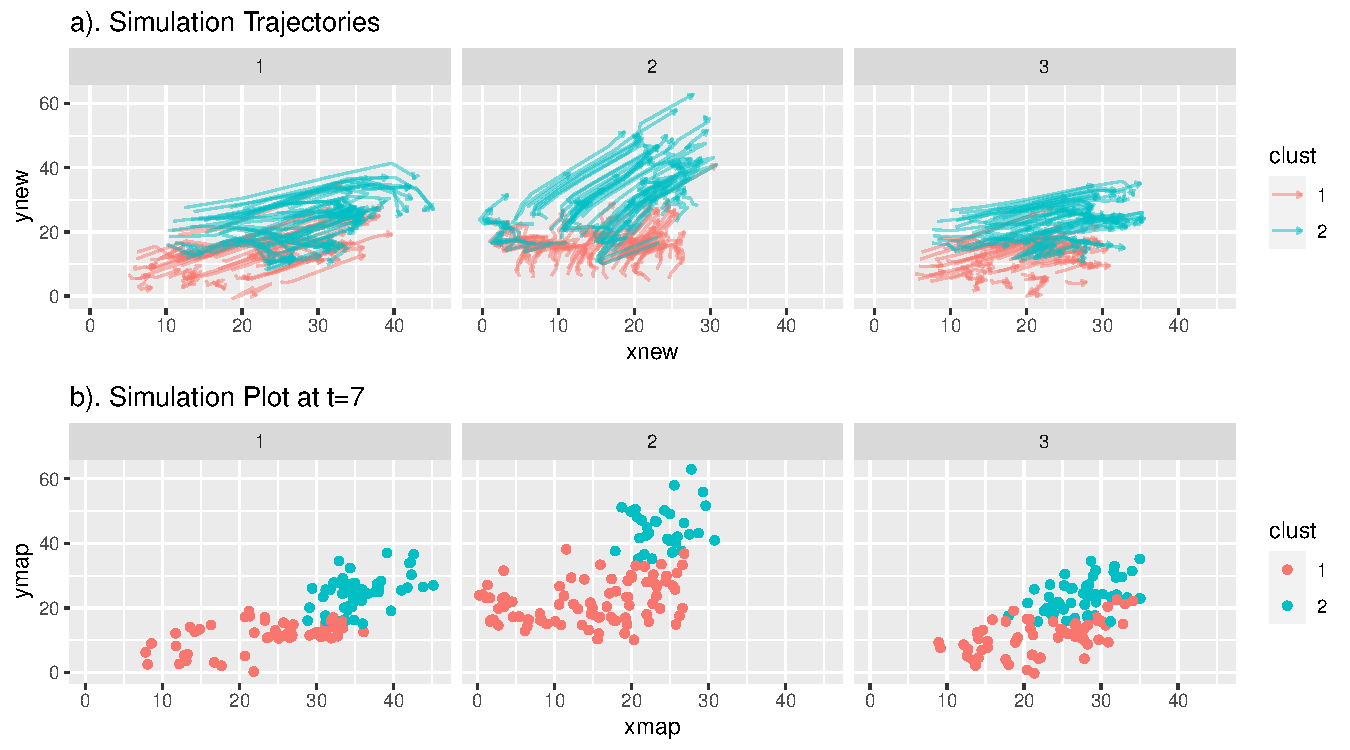
\includegraphics[width=\linewidth,]{spatio-temporal-model-arctic-sea-ice_files/figure-latex/all-combine-1} 

}

\caption{a). Trajectory Plots for each Simulated Data Set b). Clusterings of Observed Data on Final Day of Data Set}\label{fig:all-combine}
\end{figure}

Now our proposed spatio-temporal clustering method, using a bounding
box, is performed on each of the simulated datasets. Since the true
number of clusters is two, two is used as the \(k\) input in the k-means
clustering algorithm. The results are shown at two different time
points. We first plotted the k-means determined cluster on the initial
grid to visualize how well our method performs when we can see the true
clusterings. A majority of points are clustered correctly, however,
there are a number of misclassified points in each simulation, mostly
occurring along the border between clusters and along the edges. More
interestingly, the clusters are visualized on the last day of the week
to see if the clusters determined by the bounding box can distinguish
movement over time. In \cref{fig:all-clus}, there are distinguishable
boundaries between clusters for each of the simulations. Thus, by
clustering using the movement features of a trajectory, we are able to
distinguish the different movement patterns of the data with a clearly
defined boundary. Some of the misclassifications on the original grid
may be due to the value of the underlying process that was added to get
the new location. This value was determined by the closest grid cell of
the underlying process by Euclidean distance. If a point eventually
becomes closer to the other cluster, that cluster's underlying process
values are then added to cause the movement. Hence, it will eventually
start to move like the other cluster. So, if a point spends more time
moving like cluster 1 than cluster 2, as an example, it will most likely
be classified as cluster 1, even if that was not the initial cluster
assignment.

\hypertarget{interpolation-method}{%
\subsection{Interpolation Method}\label{interpolation-method}}

The same simulated data are also used to check the performance of our
spatio-temporal interpolation model. For each of the simulations,
another week of data is similarly simulated and clustered. Polygons for
each cluster are created and then the intersection polygons for each
weeks clusters are found. Once again, intersections represent the
spatio-temporal neighbors of the data within that intersection. Next,
10\% of the data for the first week are randomly assigned to be missing.
Then a univariate model for each coordinate and a bivariate model are
developed to obtain our estimates of the missing locations.

In order to have a baseline method for comparison, we also used linear
interpolation on the same data. Linear interpolation estimates an
objects unknown location along a straight-line path between two known
locations. It has been shown to work well for trajectories that follow a
straight-line path and sampled at a high rate. On the other hand, it
tends to underperform when a trajectory follows a curved path or is not
heavily sampled \citep{wentz_comparison_2003, guo_improved_2021}.
Another method used for comparison is similar to our proposed method,
except now the intersections are ignored (overall model). Instead a
model was developed using all known points for \(t-1\), \(t\), and
\(t+1\) (this essentially ignores the non-stationarity aspect of our
data). The Root Mean Square Error (RMSE) for each simulation and
interpolation method can be found in \cref{tab:results-table-by-clust}.

Our interpolation method never outperform linear interpolation. Further,
only in Simulation 3 does running the model within each intersection
perform better than the overall model. However, since each cluster was
created with different parameter values,
\cref{tab:results-table-by-clust} breaks out the RMSE calculations by
cluster to see if there are different areas where our proposed method
may perform better. If just strictly comparing our proposed univariate
method to linear interpolation, linear interpolation always performs
better in Simulation 1 and Simulation 3. In Simulation 2, our method
outperforms linear interpolation for \(y\) in cluster 2. For Simulation
2 in \cref{fig:traj-wrap}, the \(y\)-values of cluster 2 are more spread
out and curved than the other clusters in the simulation. The other
simulations may have some curvature, but samples are taken closer
together, or the data may be spread out but mostly linear. Nonetheless,
the performance of linear interpolation is not surprising as there are
long periods of linear movement in each of the simulations, so the
results may be dependent on what points were randomly removed.
Additionally, linear interpolation can not estimate the first or last
point of a trajectory, so there are fewer predicted locations used to
calculate the RMSE. Thus, these simulations show that linear
interpolation generally outperforms our univariate method, but it shows
promise with curved data that may not be highly sampled.

The results regarding intersection creation are mixed, with creating
intersections only being beneficial for Simulation 3. However, these
results may be impacted by some of the intersections not containing much
data, which may impact model development. Finally, our bivariate method
never outperforms our proposed univariate method, which makes sense as
\(x\) and \(y\) were simulated separately.

\begin{table}

\caption{\label{tab:results-table-by-clust}RMSE for Interpolation Methods}
\centering
\begin{tabular}[t]{lllrrllrr}
\toprule
\multicolumn{1}{c}{} & \multicolumn{2}{c}{Linear} & \multicolumn{2}{c}{Univariate Intersection} & \multicolumn{2}{c}{Overall Univariate} & \multicolumn{2}{c}{Bivariate} \\
\cmidrule(l{3pt}r{3pt}){2-3} \cmidrule(l{3pt}r{3pt}){4-5} \cmidrule(l{3pt}r{3pt}){6-7} \cmidrule(l{3pt}r{3pt}){8-9}
 & $X$ & $Y$ & $X$ & $Y$ & $X$ & $Y$ & $X$ & $Y$\\
\midrule
\addlinespace[0.3em]
\multicolumn{9}{l}{\textbf{Simulation 1}}\\
\hspace{1em}Overall & 1.04 & 1.23 & 1.500 & 1.510 & 1.43 & 1.29 & 1.540 & 1.670\\
\hspace{1em}Cluster 1 & 0.82 & 1.16 & 1.410 & 1.580 & 1.54 & 1.28 & 1.410 & 1.770\\
\hspace{1em}Cluster 2 & 1.19 & 1.27 & 1.570 & 1.470 & 1.35 & 1.29 & 1.630 & 1.590\\
\hspace{1em}Coverage &  &  & 0.257 & 0.271 &  &  & 0.014 & 0.014\\
\hspace{1em}Average SD &  &  & 0.383 & 0.351 &  &  & 0.016 & 0.035\\
\addlinespace[0.3em]
\multicolumn{9}{l}{\textbf{Simulation 2}}\\
\hspace{1em}Overall & 1.45 & 1.54 & 1.540 & 1.550 & 1.47 & 1.49 & 1.630 & 1.580\\
\hspace{1em}Cluster 1 & 1.32 & 1.33 & 1.700 & 1.640 & 1.66 & 1.6 & 1.800 & 1.720\\
\hspace{1em}Cluster 2 & 1.5 & 1.61 & 1.500 & 1.520 & 1.4 & 1.45 & 1.570 & 1.540\\
\hspace{1em}Coverage &  &  & 0.214 & 0.196 &  &  & 0.000 & 0.000\\
\hspace{1em}Average SD &  &  & 0.349 & 0.378 &  &  & 0.001 & 0.001\\
\addlinespace[0.3em]
\multicolumn{9}{l}{\textbf{Simulation 3}}\\
\hspace{1em}Overall & 0.95 & 0.92 & 1.410 & 1.400 & 1.46 & 1.51 & 1.430 & 1.510\\
\hspace{1em}Cluster 1 & 1.16 & 1.1 & 1.460 & 1.480 & 1.43 & 1.44 & 1.490 & 1.510\\
\hspace{1em}Cluster 2 & 0.65 & 0.67 & 1.350 & 1.310 & 1.49 & 1.58 & 1.360 & 1.510\\
\hspace{1em}Coverage &  &  & 0.243 & 0.311 &  &  & 0.014 & 0.000\\
\hspace{1em}Average SD &  &  & 0.319 & 0.337 &  &  & 0.001 & 0.001\\
\bottomrule
\end{tabular}
\end{table}

A benefit of using a model-based approach to interpolate missing
locations is that we are able to determine the uncertainty of the
estimate. To do so, for the univariate model, conditional draws of the
unobserved values given the observed values are used to quantify the
uncertainty. This is accomplished by exploiting an advantage of
Vecchia's Approximation that approximate draws from a Gaussian Process
model can be made through the inverse Cholesky Factor
\citep{guinness_permutation_2018}. Therefore, for each model, 30
simulations of predictions are conducted to calculate the standard
deviation. For our proposed bivariate method with INLA, the standard
deviation of the estimates are computed using the posterior marginals.
The standard deviation values can then be used to create an interval of
our estimates. The intervals are found by \(\hat{x} \pm (2*sd_x)\) and
\(\hat{y} \pm (2*sd_y)\), where \(\hat{x}\) and \(\hat{y}\) are the
predictions, and \(sd_x\) and \(sd_y\) are the standard deviations of a
prediction. Next, we found the proportion of the intervals that contain
the true value, otherwise known as coverage. For each simulation the
coverage can be found in \cref{tab:results-table-by-clust} along with
the average standard deviation values to show typical interval width.
The proportions in this table are low, mainly in the 20\%-30\% range for
the univariate model and \textless1\% for the bivariate model. The
standard deviation values in \cref{results-table-by-clust} are also low,
meaning there is not much variability among the predictions, thus making
intervals narrow. The low coverage values show that the model has room
for improvement in terms of prediction accuracy.

\hypertarget{results}{%
\section{Results}\label{results}}

\begin{figure}[tbp]

{\centering 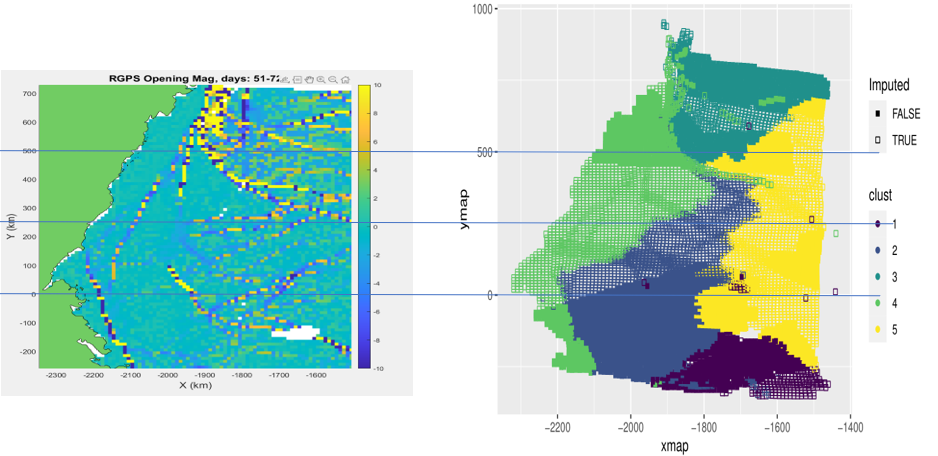
\includegraphics[width=1\linewidth,]{images/all_weeks_comp_correct} 

}

\caption{Comparison of our method to results of a previous method, which find cracks using a kinematic algorithm}\label{fig:all-week-comp}
\end{figure}

The simulation results showed some promise for our methods, so next the
methods are applied on the ice motion data set.

\hypertarget{clustering-using-all-data}{%
\subsection{Clustering Using All Data}\label{clustering-using-all-data}}

First, we used our spatio-temporal clustering method by creating
bounding boxes around each \(g_j\). Once the bounding box features were
calculated and standardized, the number of clusters were determined
using the silhouette statistic. The silhouette statistic for the full
trajectory data suggested five clusters. The results from the clustering
algorithm are shown on the right side of \cref{fig:all-week-comp}. In
this plot each of the colors represent one cluster; each of the squares
represent the last location in the data set for each \(g_j\). The
unfilled squares represent missing data at this time. We hypothesize
that cracks in the sea ice will be found along the boundaries of the
clusters. In the middle of some clusters, there are some singular points
whose cluster membership does not match its neighbors. In practicality
these points will belong to the same cluster as its neighbors and a
crack is not considered to have formed here. In the future, a
post-processing filter to address these anomalies can be developed.

To see how well our method is performing, we can compare it to other sea
ice crack detection methods. One such method plots the deformation data
using a kinematic crack algorithm using the RGPS data
\citep{peterson_evaluating_2011}. \cref{fig:all-week-comp} gives a
comparison of our bounding box clustering method and the kinematic crack
algorithm using side-by-side plots. It is important to note that the
plot of the deformation data does not represent the true ice cracks,
just the cracks determined by this method. The plots are aligned so that
their axes match up for easier comparison. The lines given in the left
figure are derived from the opening magnitude of the ice sheet. Most of
the figure has a color around zero, denoting no opening, whereas
potential cracks are found with the dark blue or yellow. Many of our
cluster boundaries match up with the cracks identified by the kinematic
crack algorithm, though our proposed method is limited by the number of
clusters. For example, on the bottom left of each plot, there is a line
that goes down and to the right. At the bottom right of both plots,
there is a line through the hole in the points. Additionally, towards
the top of each plot, there is a curved boundary that starts at the top
of the ice sheet and moves to the bottom left in a curved manner.

\hypertarget{clusterings-by-weeks}{%
\subsection{Clusterings By Weeks}\label{clusterings-by-weeks}}

Since trajectories can be long, it is also useful to look at
sub-trajectories as we lose information be clustering the whole
trajectory, which impacts results. Through some testing of our methods,
we found that by week was the smallest time period we could successfully
cluster, as anything smaller led to large changes in the clusterings
between each week (unstable). We expect the weeks to have different
clusters, but we also expect there to be some continuity between them.
The clusters by week can be found in \cref{fig:by-week-cluster-plot},
where can see some similarities in clusters over time. In the clusters
for week 1 and week 2, there is a line moving from the top and down to
the left, which is seen in the kinematic crack algorithm, but not in
\cref{fig:ex-result}. This is an example of where clustering the
sub-trajectories may provide additional information. These clusters for
each week were used to develop the intersections used for interpolation.

\begin{figure}[tbp]

{\centering \includegraphics[width=\linewidth,]{spatio-temporal-model-arctic-sea-ice_files/figure-latex/by-week-cluster-plot-1} 

}

\caption{Results of Clustering using Bounding Box Method by Week}\label{fig:by-week-cluster-plot}
\end{figure}

\hypertarget{interpolation-methods}{%
\subsection{Interpolation Methods}\label{interpolation-methods}}

\begin{figure}[tbp]

{\centering 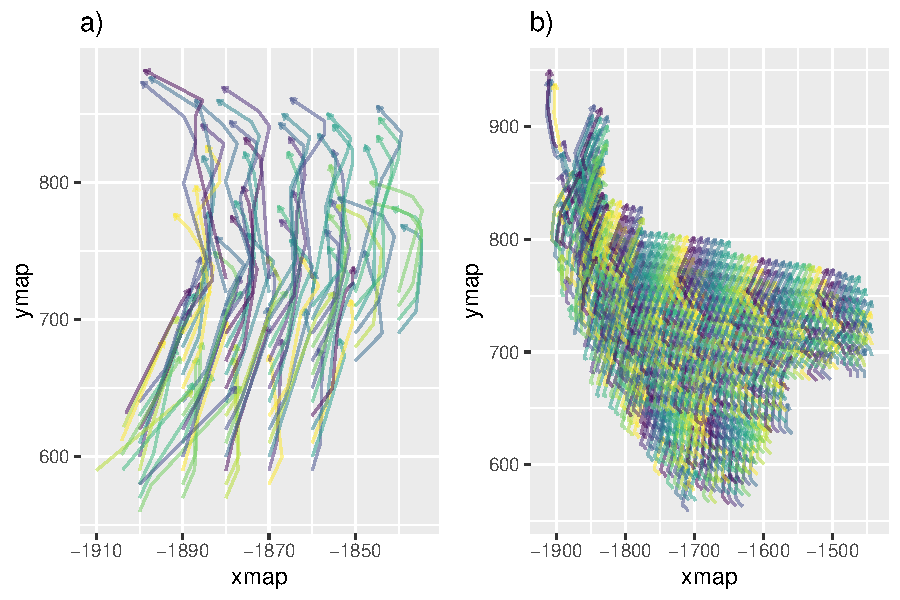
\includegraphics[width=\linewidth,]{spatio-temporal-model-arctic-sea-ice_files/figure-latex/int-best-plots-1} 

}

\caption{Trajectories for a) Week 2 Cluster 5, where linear interpolation performs best and b) Week 2 Cluster 1, where our proposed univariate method peforms best.}\label{fig:int-best-plots}
\end{figure}

Next, we tested our spatio-temporal interpolation method on the ice
motion data set to see how it performs on real data. We did not estimate
the already missing data for validation purposes. For cross validation,
we can create a model for each intersection and time combination. The
intersections were found using the clusters in
\cref{fig:by-week-cluster-plot}. In each intersection and time
combination, 10\% of the known data was removed. Next, we found all the
observed data in that intersection for \(t-1\), \(t\), and \(t+1\) to
obtain the spatio-temporal neighbors. Then, using the observed data, the
univariate and bivariate models were fit and used to estimate the points
assigned to be missing. This was done for all intersection and time
combinations for the three weeks. The RMSE for each week can be found in
\cref{tab:results-table2}. Additionally, linear interpolation and the
overall model method were performed on the same missing data for
comparison. However, since linear interpolation is unable to estimate
data without a point before and after (essentially the beginning or end
of the week), it is not exactly a one-to-one comparison. Also, for the
overall model, due to the log-likelihood failing to converge, a model
was only able to be developed for two out of the seven days in Week 1.
Hence, the week 1 RMSE value for this week is not useful for comparison.
In \cref{tab:results-table2}, linear interpolation outperforms the other
methods except for the \(y\)-values in week 1.

\begin{table}

\caption{\label{tab:results-table2}RMSE for Interpolation Methods}
\centering
\begin{tabular}[t]{lllrrllrr}
\toprule
\multicolumn{1}{c}{} & \multicolumn{2}{c}{Linear} & \multicolumn{2}{c}{Univariate Intersection} & \multicolumn{2}{c}{Univariate Overall} & \multicolumn{2}{c}{Bivariate} \\
\cmidrule(l{3pt}r{3pt}){2-3} \cmidrule(l{3pt}r{3pt}){4-5} \cmidrule(l{3pt}r{3pt}){6-7} \cmidrule(l{3pt}r{3pt}){8-9}
 & $X$ & $Y$ & $X$ & $Y$ & $X$ & $Y$ & $X$ & $Y$\\
\midrule
\addlinespace[0.3em]
\multicolumn{9}{l}{\textbf{Week 1}}\\
\hspace{1em}RMSE & 1.53 & 4.18 & 3.250 & 3.210 & 3.09 & 2.88 & 3.170 & 7.720\\
\hspace{1em}Coverage &  &  & 0.256 & 0.293 &  &  & 0.005 & 0.018\\
\hspace{1em}Average SD &  &  & 0.788 & 0.834 &  &  & 0.016 & 0.087\\
\addlinespace[0.3em]
\multicolumn{9}{l}{\textbf{Week 2}}\\
\hspace{1em}RMSE & 2 & 1.4 & 3.140 & 3.060 & 3.2 & 3.15 & 3.190 & 3.110\\
\hspace{1em}Coverage &  &  & 0.263 & 0.298 &  &  & 0.009 & 0.015\\
\hspace{1em}Average SD &  &  & 0.751 & 0.810 &  &  & 0.026 & 0.026\\
\addlinespace[0.3em]
\multicolumn{9}{l}{\textbf{Week 3}}\\
\hspace{1em}RMSE & 1.03 & 1.21 & 3.170 & 3.090 & 3.19 & 3.15 & 3.130 & 3.040\\
\hspace{1em}Coverage &  &  & 0.246 & 0.263 &  &  & 0.004 & 0.007\\
\hspace{1em}Average SD &  &  & 0.760 & 0.796 &  &  & 0.010 & 0.019\\
\bottomrule
\end{tabular}
\end{table}

However, when looking at the trajectory plot in \cref{fig:trajectories},
some of the trajectories in the plot are more linear than others (ie.
different movements defined by the clusters). Based on our simulation
study, our univariate method shows improvement over linear interpolation
on curved and less-sampled trajectories. Thus, the RMSE values are also
broken out by cluster, as these are the groups of movement patterns in
the data. These values can be found for each week in
\cref{tab:results-clust-actual}. Once again, linear interpolation
generally outperforms our proposed methods, but there are two
exceptions. For Week 1 and Week 2, linear interpolation performs worse
than our proposed linear model in Cluster 1. In
\cref{fig:by-week-cluster-plot}, Cluster 1 for both of these weeks is at
the top of the plot. When comparing this cluster location to the
trajectory plot in \cref{fig:trajectories}, the top of the figure is
where the most curved movement happens with a longer distance traveled
over time. Hence, linear interpolation may not work as well here.
Further, \cref{fig:int-best-plots} zooms in on an example for week 2
where our univariate intersection method performs best (plot (a)) and
linear interpolation performs best (plot (b)).
\cref{fig:int-best-plots}a) is Cluster 1, where the observed points are
more spread out along the trajectory. On the other hand
\cref{fig:int-best-plots}b) has small, linear movement, which is why
linear interpolation performs best.

As previously stated, though the RMSE for the overall univariate model
was lower than the univariate intersection model in week 1, this only
represents one day's worth of data. Overall, when comparing the two
univariate model-based approaches, we find mixed results when comparing
their performance, but the univariate intersection model performs better
more often. Our bivariate method never outperforms our univariate
intersection model. Once again, these results show that our univariate
method has some promise with non-linear and less-sampled data.

\begin{table}

\caption{\label{tab:results-clust-actual}RMSE by Cluster for Interpolation Methods}
\centering
\begin{tabular}[t]{rrrrrrrrr}
\toprule
\multicolumn{1}{c}{ } & \multicolumn{2}{c}{Linear} & \multicolumn{2}{c}{Univariate Intersection} & \multicolumn{2}{c}{Overall Univariate} & \multicolumn{2}{c}{Bivariate} \\
\cmidrule(l{3pt}r{3pt}){2-3} \cmidrule(l{3pt}r{3pt}){4-5} \cmidrule(l{3pt}r{3pt}){6-7} \cmidrule(l{3pt}r{3pt}){8-9}
Cluster & $X$ & $Y$ & $X$ & $Y$ & $X$ & $Y$ & $X$ & $Y$\\
\midrule
\addlinespace[0.3em]
\multicolumn{9}{l}{\textbf{Cluster 1}}\\
\hspace{1em}1 & 3.20 & 13.04 & 3.07 & 4.10 & 2.52 & 3.61 & 3.16 & 17.68\\
\hspace{1em}2 & 0.19 & 0.36 & 4.36 & 4.30 & 4.26 & 3.98 & 4.58 & 4.63\\
\hspace{1em}3 & 1.31 & 3.07 & 3.08 & 3.10 & 2.17 & 2.72 & 2.85 & 9.88\\
\hspace{1em}4 & 1.40 & 2.44 & 3.10 & 2.85 & 2.46 & 2.34 & 2.97 & 2.79\\
\hspace{1em}5 & 0.77 & 3.17 & 3.91 & 3.67 & 3.89 & 2.55 & 3.99 & 8.78\\
\hspace{1em}6 & 1.89 & 5.64 & 3.10 & 3.06 & 2.63 & 3.35 & 3.23 & 4.69\\
\addlinespace[0.3em]
\multicolumn{9}{l}{\textbf{Cluster 2}}\\
\hspace{1em}1 & 3.24 & 3.32 & 3.00 & 2.93 & 2.62 & 3.04 & 3.05 & 4.60\\
\hspace{1em}2 & 2.55 & 1.03 & 2.94 & 2.89 & 2.89 & 2.94 & 3.04 & 2.88\\
\hspace{1em}3 & 1.58 & 1.99 & 2.94 & 2.90 & 2.95 & 3.03 & 2.95 & 2.91\\
\hspace{1em}4 & 1.40 & 0.52 & 3.26 & 3.13 & 3.45 & 3.19 & 3.37 & 3.17\\
\hspace{1em}5 & 0.31 & 0.37 & 4.23 & 4.16 & 4.41 & 4.20 & 4.32 & 4.28\\
\addlinespace[0.3em]
\multicolumn{9}{l}{\textbf{Cluster 3}}\\
\hspace{1em}1 & 2.04 & 2.67 & 2.85 & 2.85 & 2.70 & 3.04 & 2.94 & 2.84\\
\hspace{1em}2 & 2.15 & 2.06 & 2.81 & 2.95 & 2.65 & 2.85 & 2.68 & 2.97\\
\hspace{1em}3 & 0.19 & 0.44 & 3.65 & 3.59 & 3.75 & 3.60 & 3.70 & 3.61\\
\hspace{1em}4 & 1.53 & 0.72 & 2.67 & 2.78 & 2.87 & 2.92 & 2.61 & 2.87\\
\hspace{1em}5 & 0.21 & 0.48 & 3.16 & 3.04 & 3.08 & 3.09 & 3.11 & 2.99\\
\hspace{1em}6 & 0.28 & 0.55 & 3.21 & 3.01 & 3.23 & 3.01 & 3.25 & 3.03\\
\bottomrule
\end{tabular}
\end{table}

The proportion of the prediction intervals containing the observed data,
along with the average standard deviations are given in
\cref{tab:results-table2}. These values were found in the same way as
the simulated data. The standard deviations for the univariate are
higher than what was seen with the simulated data, but the coverage is
similar (ranging from 25\%-30\%), but around the same for the bivariate
model. However, once again, none of the values are as large as desired.
The model then may need further investigation and development to
increase this, as this may be indicating something is wrong.

\hypertarget{discussion}{%
\section{Discussion}\label{discussion}}

Our bounding box clustering methods was developed to group trajectories
by their movement, and to compensate for missing data. This method was
shown, through simulations and actual data, that the boundaries of the
clusters determined by the trajectory movements provide a reasonable
estimation for the location of leads. However, a major drawback of this
method is that due to the use of k-means clustering, our method relies
on a pre-defined number, which is unknown. Furthermore, since there is a
set number of clusters, there is a limit on how many cluster boundaries,
representing leads, that can be identified. Thus, not all possible leads
will be identified. Our method suggest that other approaches should be
used to extend this method to identify higher resolution leads. Our
method does provide additional information about how the ice sheet is
moving, which may also be important when developing climate models.

Through our simulated and ice motion data, we have demonstrated some
situations where our proposed univariate, and even bivariate,
interpolation method may be useful. First, both method take into account
the non-stationarity of the data. The univariate intersection model
generally shows slight improvements over the overall univariate model.
Instances where the univariate intersection models underperforms the
overall model may be due to lack of data to develop the model at smaller
intersections. Secondly, goth of our proposed methods are able to
estimate missing location on the first and last day of a data set, which
is impossible with linear interpolation. Third, our univariate
intersection method showed improvements over linear interpolation for
curved and low-sampled data. Finally, since we are creating a model, we
are able to calculate an uncertainty measure with the predictions.
Despite these benefits, linear interpolation performs better in most
cases. So the additional information about movement does not seem to
provide any benefit of the trajectories are linear and we are only
interested in location estimation.

A drawback of our method for finding spatio-temporal neighbors is that
if an object is not located within an intersection, it is removed from
the data used to develop the models. Thus, we could be losing valuable
information for model development to obtain the estimates. Typically
this only happens to \(g_j\) on the edges of the ice sheet.

When developing the univariate models with the Vecchia Approximation,
some other issues arise. The first is that for some models, the
log-likelihood fails to converge (only happens with the ice data). This
seems to happen if \(\sigma^2\) and \(\phi\) become exceptionally large,
which also means they no longer make sense practically. For example,
even when the model converges, \(\phi\) is in the thousands. Meaning the
data is not changing much over space, so the model may struggle for
intersection that are small and do not move much. Additionally, for some
models, singularity is an issue and an approximate solution is used in
the development of the model, though this still produces a model.

The proposed bivariate model, while generally performing the worst in
terms of RMSE, is the only model tested that provides an estimate for
each missing data point. The only issue with developing these models
happens if there is no variation in time. Meaning that when using
\(t-1\), \(t\), and \(t+1\), only one of those days has observed data.
When this happens the model does not produce an error like it does for
the univariate model, instead it estimates parameters of 0 or infinity
which return very poor predictions.

Finally as shown in \cref{tab:results-table2}, the coverage for both the
univariate and bivariate models are low. So while the univariate method
may show some promise with curved data, more investigation needs to be
done as this coverage may be pointing to some flaw in our model that
needs to be further investigated.

\hypertarget{conclusion}{%
\section{Conclusion}\label{conclusion}}

Sea ice plays a vital role in the Earth's energy balance, as when leads
form in the ice, warm air from the ocean is released into the
atmosphere. In order to determine where these leads may form using only
the movement of an ice sheet, a bounding box is created around each
trajectory. The features of the bounding box are used as input into
k-means. Once each \(g_j\) is assigned a cluster, a plot of the results
is created where the cluster boundaries would be the location where
leads may form. This method found similar leads as other ice crack
detection methods. Next, using the information from spatio-temporal
neighbors of the missing points, we developed a univariate and bivariate
model for interpolation of the missing points. While linear
interpolation typically outperforms our proposed methods, the univariate
model showed some promise with nonlinear and low-sampled data.

In the future, more work needs to be done on the univariate model
development for interpolation to facilitate convergence in a wider range
of situations. Additionally, both the univariate and bivariate models
need to be further investigated to increase coverage, which may also
help with the convergence issues. Finally, at the moment, our
interpolation method is a two-step process: find clusters and create a
model. Eventually, we would like to turn this into a one-step process,
potentially using Voronoi tessellations and a piecewise Gaussian
Process.

\bibliographystyle{agsm}
\bibliography{bibliography.bib}


\end{document}
